\section{Pattern Formation \& Non-Reciprocal Phase Transitions}

In stat mech, we generally understand a phase transition as a discontinuity in a free energy, or where the free energy of a system changes form (e.g. from a single to a double well). How do we understand phase transitions in systems where we cannot write down an energy?

\subsection{Swift-Hohenberg Model}
We consider the dynamical equation (a non-linear PDE):
\begin{equation}\label{eq:swifthohen}
    \p_t u(x, t) = ru - (1 + \lambda_c^2\nabla^2)^2u - u^3
\end{equation}
What the $\lambda_c^2 \nabla^2$ term does is favour the system towards an oscillation a wavelength $\lambda_c$. It is easy to reinterpret this equation as the variation of a potential:
\begin{equation}
    \p_t u = -\frac{\delta V}{\delta u}
\end{equation}
Where:
\begin{equation}
    V = \int dx \left(-\frac{1}{2}ru^2 + \frac{1}{4}u^4 + \frac{1}{2}\left[[\lambda_c^2 \nabla^2 + 1]u\right]^2\right)
\end{equation}
where in we see the $\lambda_c$ term vanishes if we consider $u = e^{iqx}$ with $q = \frac{1}{\lambda_c}$. But note that Eq. \eqref{eq:swifthohen} has an additional solution, namely $u = 0$.

To this end, we have to do a linear stability analysis around the solutions (we skip some steps - this is done in the text and also in your homework), and see if the perturbation grows or decays in time. So, we consider:
\begin{equation}
    u = u_0 + \delta u(x, t) = \delta u(x, t)
\end{equation}
where we have taken the $u_0 = 0$ solution. We can now linearize around the perturbation:
\begin{equation}
    \p_t \delta u = L\delta u + O((\delta u)^2) = \underbrace{[r - (1 + \lambda_c^2\nabla^2)^2]}_{L}\delta u + O((\delta u)^2)
\end{equation}
If we Fourier transform the $L$:
\begin{equation}
    L(q) = [r - (1 - q^2\lambda_c^2)^2]
\end{equation}
We can now write down the exponential behaviour of $\delta u(q)$:
\begin{equation}
    \delta u(q) = e^{\sigma(q) t}
\end{equation}
where:
\begin{equation}
    \sigma(q) = (r - 1) + 2\lambda_c^2 q^2 - q^4\lambda_c^4
\end{equation}
So - we are interested in the sign of $\sigma(q)$, because if $\sigma(q)$ is negative then $u$ is stable ($\delta u \to 0$), and if $\sigma(q)$ is positive then $u$ is unstable ($\delta u \to \infty$). To this end, let us plot $\sigma(q)$, which will be a symmetric function around $q = 0$:

\begin{center}
    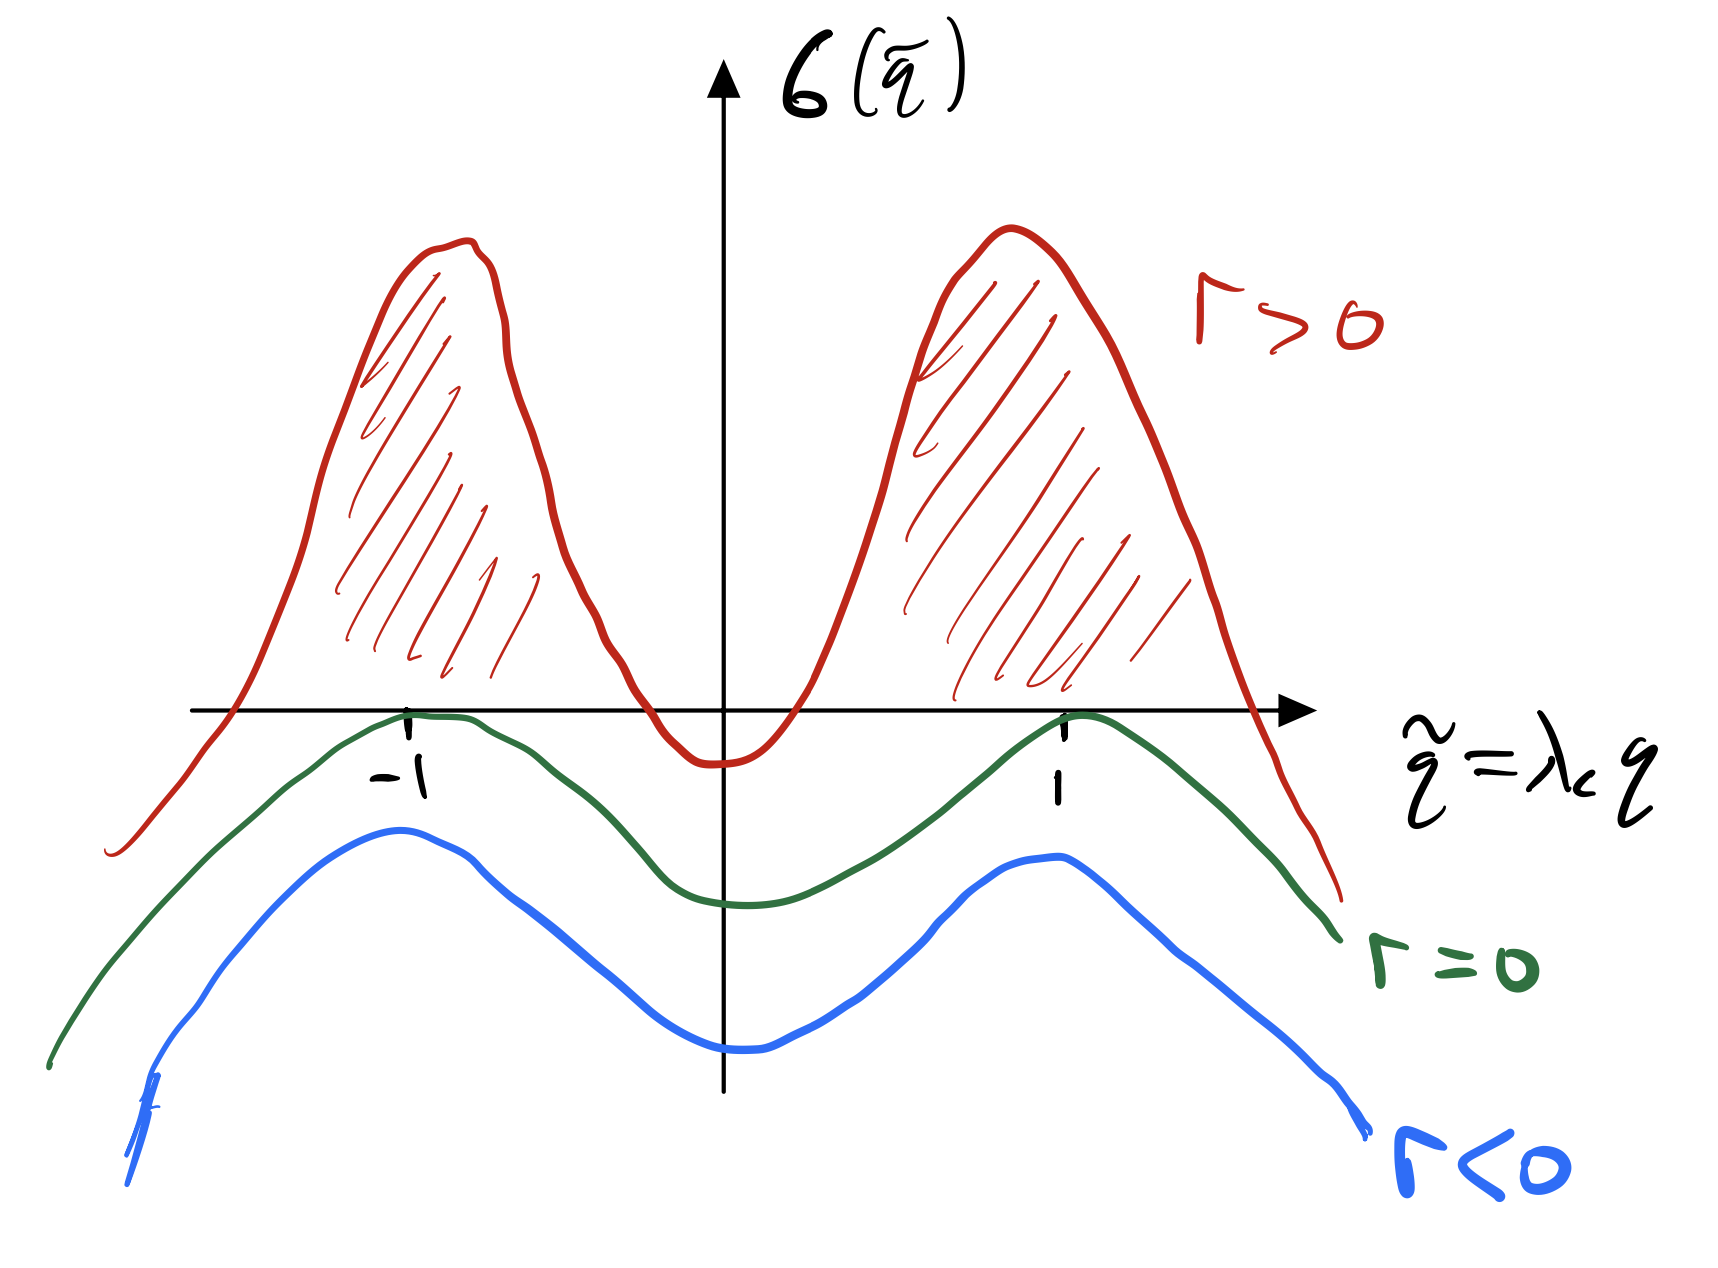
\includegraphics[scale=0.3]{Lectures/Images/lec18-sigmaq.png}
\end{center}

We find at the maxima:
\begin{equation}
    \sigma(\tilde{q} = \pm 1) = (r - 1) + 2 - 1 = r
\end{equation}
So depending on the sign of $r$, we have stability or instability, with wavelength selection at $\tilde{q} = 1$ or at $q_c = \frac{1}{\lambda_c}$.

If we study perturbative solutions to Eq. \eqref{eq:swifthohen}, we find:
\begin{equation}
    u(x, t) = \underbrace{a_1}_{\sqrt{\frac{4}{3}r}}\cos(x) + \mathcal{O}(r^{3/2})\cos(3x)
\end{equation}
Much like in critical phenomena we expand in $T - T_c$, we here expand in $r$. We can look at the amplitude of the $u$:

\begin{center}
    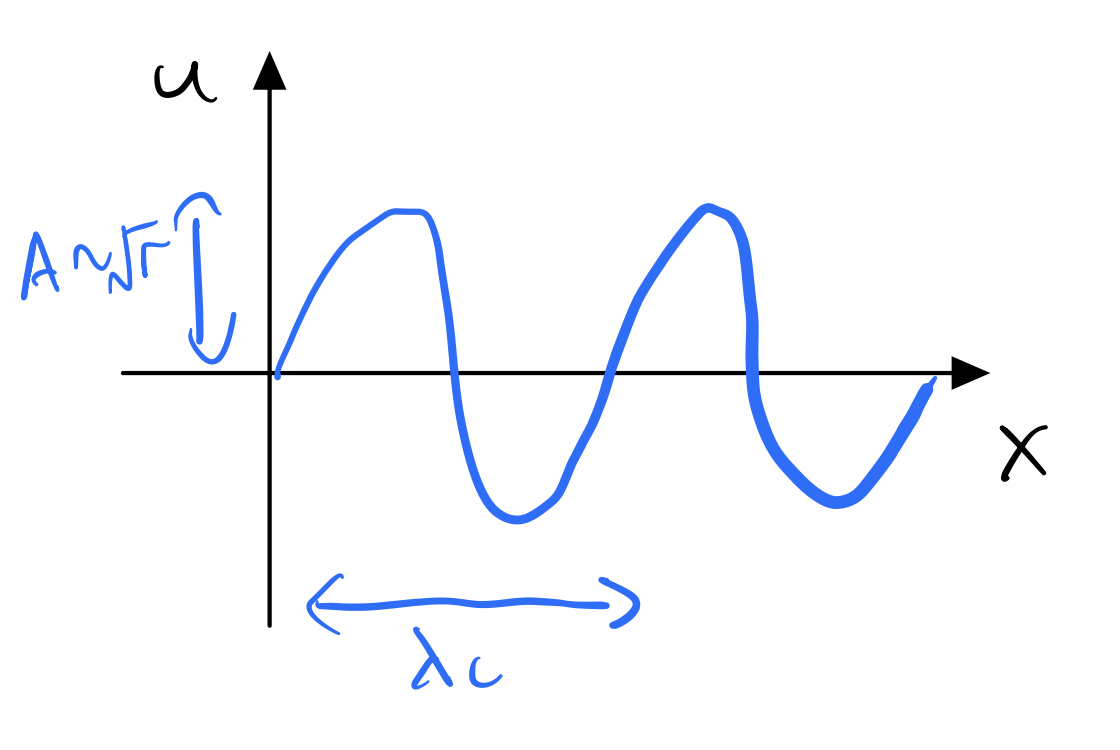
\includegraphics[scale=0.35]{Lectures/Images/lec18-ux.png}
\end{center}

Where we find a pitchfork bifurcation:

\begin{center}
    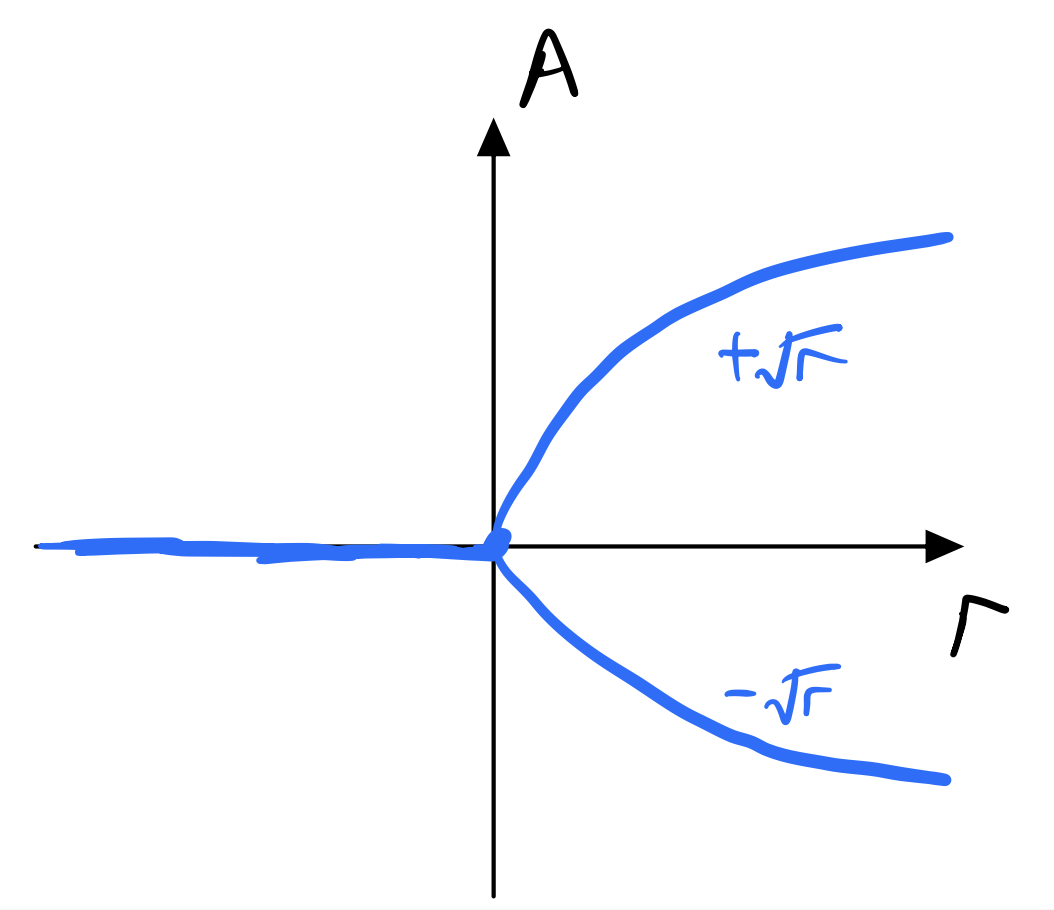
\includegraphics[scale=0.35]{Lectures/Images/lec18-Abifurcation.png}
\end{center}

Much like you have seen in the Ising model. How do we understand this? We are looking at the solutions:
\begin{equation}
    u(x, t) \sim A(x, t)e^{iq_c x} + \text{c.c.}
\end{equation}
where $e^{iq_c x}$ is dictated by the fastest growing mode. We have oscillation dictated by $q_c$, but we can also have a modulation of the amplitude (slower than dictated by $q_c$) dictated by $A(x, t)$, giving a more full description of the problem:

\begin{center}
    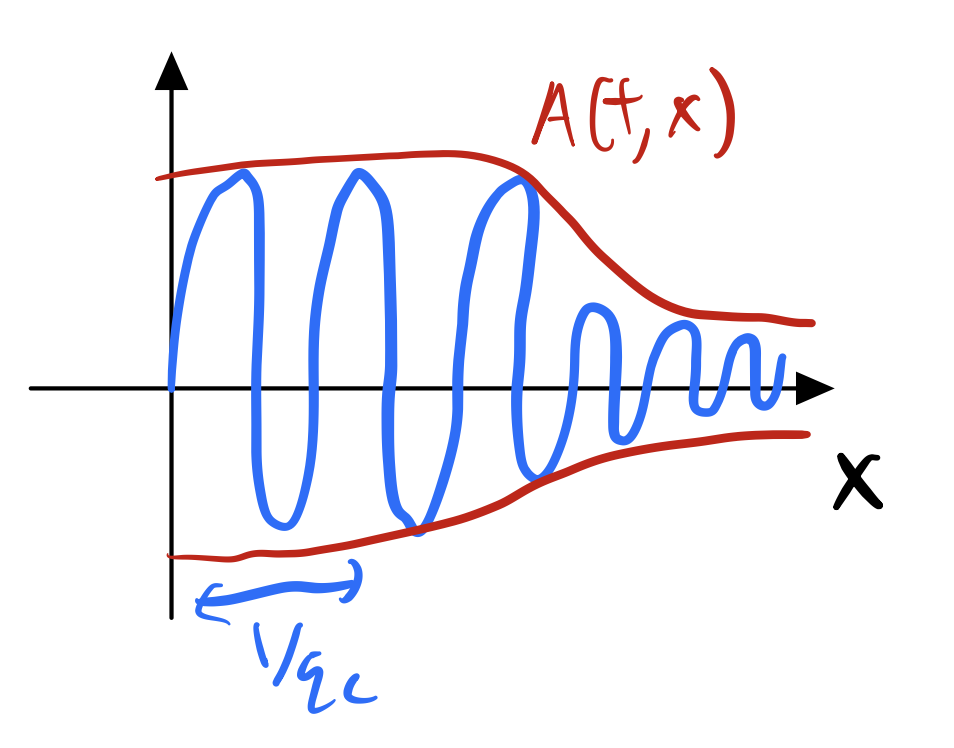
\includegraphics[scale=0.35]{Lectures/Images/lec18-Amodulation.png}
\end{center}

What we can do is consider a complex amplitude $A = ae^{i\phi}$ (with $a = \abs{A}$) and consider a shift to the phase:
\begin{equation}
    \phi \to \phi + \Delta \phi
\end{equation}

\begin{center}
    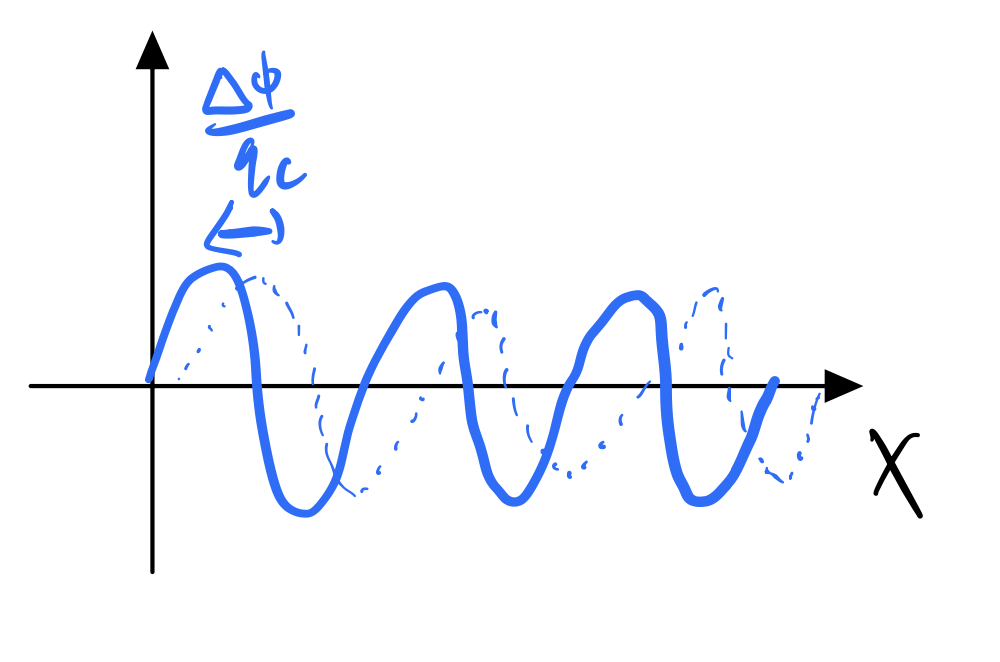
\includegraphics[scale=0.35]{Lectures/Images/lec18-phasediff.png}
\end{center}

This causes a translation of the pattern in time (known as limit cycles). Notice that in our model we have a transition from no pattern (in our case at $r < 0$ where $A = 0$) to a periodic pattern (at $r > 0$ where $A = \pm\sqrt{r}$) - spontaneous translational symmetry breaking - controlled by $r$.

\subsection{Non-reciprocal Swift-Hohenberg Model}
We want to introduce non-reciprocity into our model. We do this by introducing two fields labelled by $a = 1, 2$ and modify the $r$ coefficient to be a matrix $\e_{ab}$, so our dynamical equation becomes:
\begin{equation}
    \p_t u_a(x, t) = \e_{ab}u_b - (1 + \lambda_c^2\nabla^2)^2u_a - u_a^3
\end{equation}
Now, we notice that if $\e_{ab} \neq \e_{ba}$, it is the case that:
\begin{equation}
    \p_t u \neq -\frac{\delta V}{\delta u}
\end{equation}
because the antisymmetric part of $\e_{ab}$, i.e.:
\begin{equation}
    \e_{ab}^o = - \e^o_{ba}
\end{equation}
then:
\begin{equation}
    \e^o_{ab}u_a u_b = 0
\end{equation}
(as we multiply an antisymmetric object with a symmetric one) so while $\e_{ab}u_b$ can exist as a term in the equation of motion, there is no way of writing this down in the potential.

Note that without the cubic term, we would have just an equation of motion that describes a 1-D crystal. But the cubic/nonlinear term allows us to describe the transition between a 1-D crystal and no crystal formation.

We consider:
\begin{equation}
    \e =\m{\e_{11} & \e_{12} \\ \e_{21} & \e_{22}} =  \m{\e_{0} & \e_{12} \\ \e_{21} & \e_0}
\end{equation}
Now, let us write:
\begin{equation}
    \e_{12} = \e_+ + \e_-
\end{equation}
\begin{equation}
    \e_{21} = \e_+ - \e_-
\end{equation}
i.e. writing the off-diagonal components of the tensor in terms of the symmetric and antisymmetric parts. Now let us write:
\begin{equation}
    u_a(x) = A_a(x)e^{ik_c x} + \text{c.c.}
\end{equation}
Which allows us to write the equations of motion for $A_a$:
\begin{equation}
    \p_t A_1 =  \e_0 A_1 + \e_{12}A_2 - g\abs{A_1}^2A_1
\end{equation}
\begin{equation}
    \p_t A_2 = \e_0 A_2 + \e_{21}A_1  - g\abs{A_2}^2A_2
\end{equation}
which we can either derive or argue from symmetry considerations based on the equation of motion for $u$. 

We work in the regime where:
\begin{equation}
    \e_0 \gg \e_- \gg \e_+
\end{equation}

If we simulate this, we find that $u_1, u_2$ move with the same velocity if they are off by a phase. If the phase offset is zero, the pattern is fixed. So, the model allows for three cases - states where the patterns do not form, states where patterns form but they are static, and states where the pattern form and are dynamic; they spontaneously break the symmetry and move together the left/right.

\begin{center}
    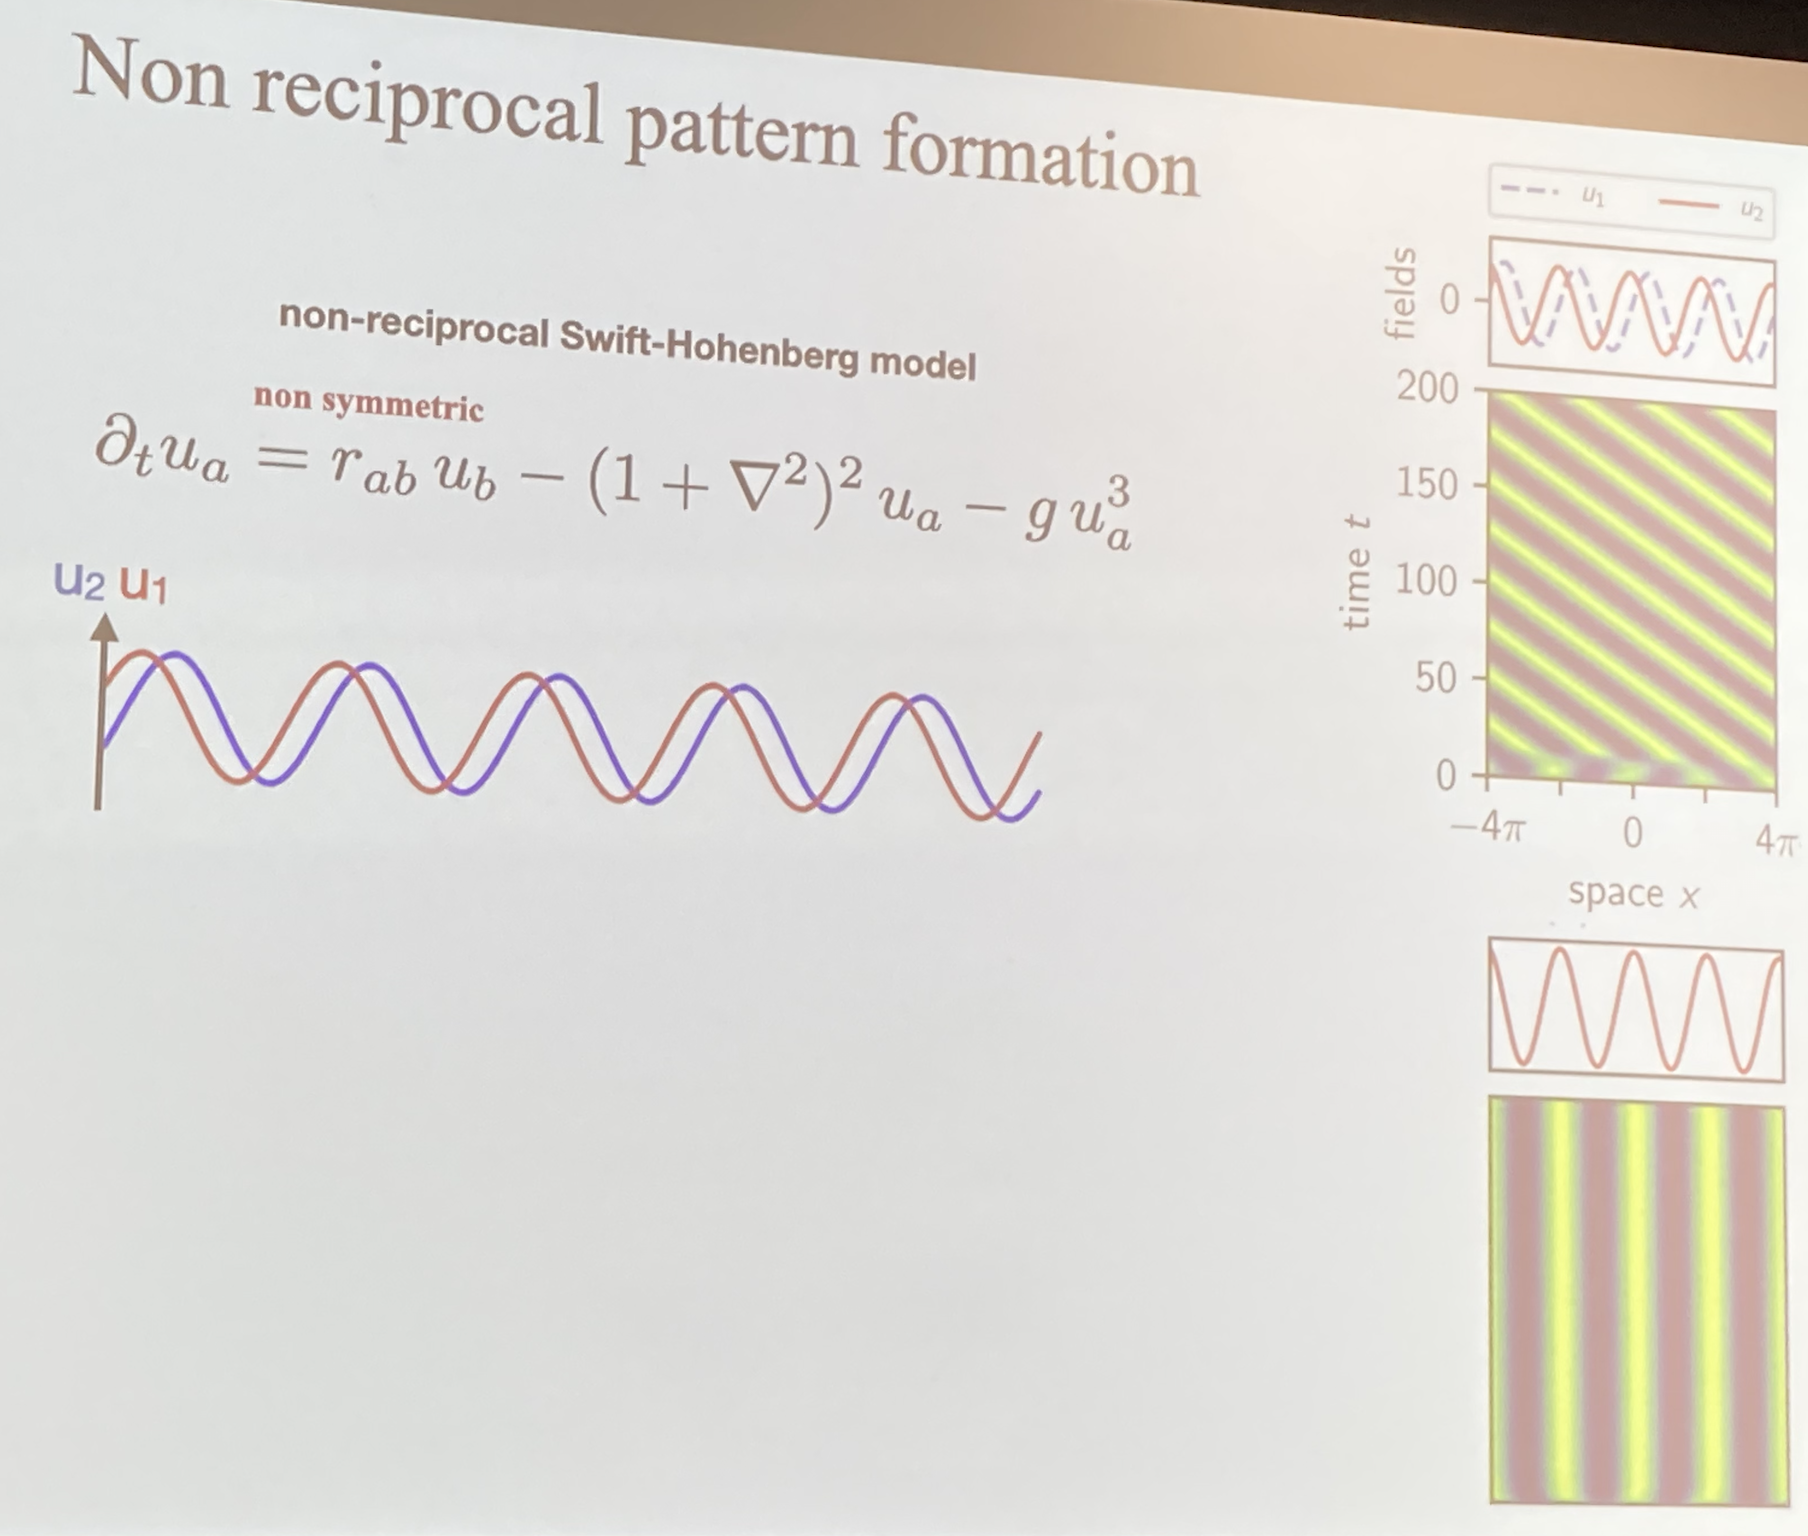
\includegraphics[scale=0.3]{Lectures/Images/lec18-wavedynamics.png}
\end{center}

Let us look at the steps of the calculation to figure out the phase diagram of this model (you will flesh out the steps in the homework).

\subsection{Deriving the Motion/Phase Diagram}
Let us write:
\begin{equation}
    A_1 = a_1e^{i\phi_1}
\end{equation}
\begin{equation}
    A_2 = a_2e^{i\phi_2}
\end{equation}
And plug them into our coupled differential equations for $A_1, A_2$. If we then parameterize:
\begin{equation}
    \Delta \phi = \phi_2 - \phi_1,\quad \bar{\phi} = \phi_2 + \phi_1
\end{equation}
where $\Delta \phi$ is the phase difference, $\bar{\phi}$ is the mean of the phases. We find a beautiful set of equations (to leading order in $\Delta \phi$):
\begin{equation}
    \p_t \Delta \phi = \alpha \Delta \phi - \beta \Delta \phi^3
\end{equation}
\begin{equation}
    \p_t \bar{\phi} = \gamma \Delta \phi
\end{equation}
where you will also derive how $\alpha, \beta, \gamma$ depend on $\e_{ab}$:
\begin{equation}
    \alpha = 2[\e_-^2 - \e_+\e_0]/\e_0
\end{equation}
\begin{equation}
    \gamma = 2\e_-
\end{equation}
and $\beta > 0$. Note that without linearization, the second equation would read $\p_t \bar{\phi} = \gamma \sin(\Delta \phi)$ so we have indeed linearized. 

If we look at the first equation, we have standard pitchfork bifurcation; indeed the set of equations for $\Delta \phi, \bar{\phi}$ is known as \emph{drift pitchfork bifurcation}.

Let's look at stable solutions to the first equation:
\begin{equation}
    0  = \alpha\Delta \phi - \beta \Delta \phi^3 = \Delta\phi(\alpha - \beta\Delta \phi^2)
\end{equation}
so we have solutions:
\begin{equation}
    \Delta \phi = 0, \Delta \phi = \pm\sqrt{\frac{\alpha}{\beta}}
\end{equation}
When $\alpha < 0$, we only have the $\Delta \phi = 0$ solution, and when $\alpha > 0$ we have that the $\pm\sqrt{\frac{\alpha}{\beta}}$ are the minima.

Looking at the second equation, for $\Delta \phi = 0$ we have that $\p_t \bar{\phi} = 0$ (so no motion of the mean) while for $\Delta \phi = \pm\sqrt{\frac{\alpha}{\beta}}$ we have motion of the mean to the right/left. The absolutely crucial thing to notice here is that if we view the motion of $\m{\Delta \phi & \bar{\phi}}^T$, the first component alone may admit a variational structure (as you have seen with magnetization in the Ising model), but together they do not admit such a structure! Also note that the dynamics here manifestly break the mirror symmetry - the dynamics are chiral.

If we linearize, we have the matrix form:
\begin{equation}
    \p_t \m{\Delta \phi \\ \bar{\phi}} = \m{\alpha & 0 \\ \gamma & 0}\m{\Delta \phi \\ \bar{\phi}}
\end{equation}

We have the phase diagram:

\begin{center}
    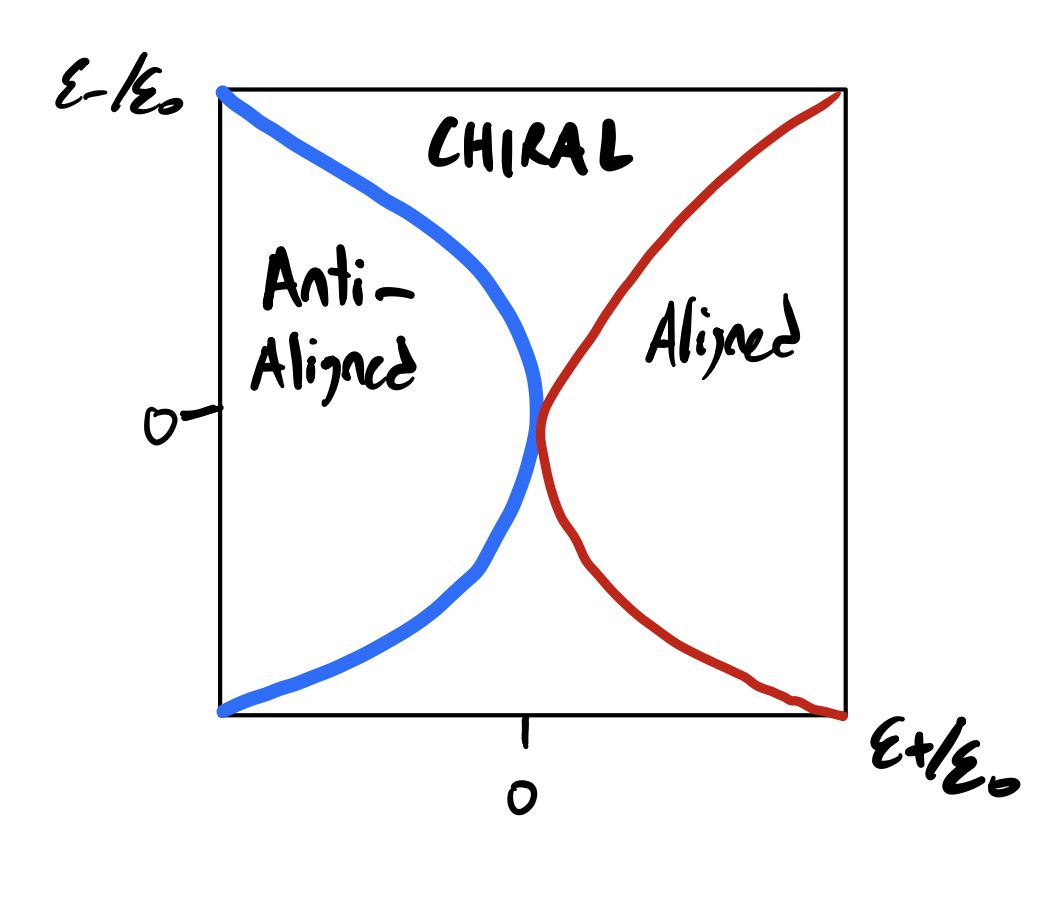
\includegraphics[scale=0.35]{Lectures/Images/lec18-phasediagram.png}
\end{center}

We can study the exceptional points; namely as $\alpha \to 0$ the eigenvectors of $\m{\alpha & 0 \\ \gamma & 0}$ coalesce/become collinear. (Why is the second column always zero? $\bar{\phi}$ corresponds to a uniform translation of the pattern, and it never plays a role in determining the phase difference $\Delta \phi$). Note that whenever we diagonalize this matrix, we have one eigenvalue that is always zero, which corresponds to the Goldstone mode. But at the exceptional point the other (nonzero) eigenvalue becomes zero, and that is where the transition happens. The onset of the bifurcation occurs at the exceptional point of the Jacobian, and then we can derive the phase diagram of this system.

\subsection{Non-Reciprocal Flocking Models}
Although it is more complicated, we can also see such a non-reciprocal phase transition arise in a Flocking model - we can take the Vicsek model, add two types of populations, and make their interactions non-reciprocal. Unlike the standard Vicsek model where the flock travels in a particular direction uniformly, in the non-reciprocal model we have that the two populations rotate, with the order parameters rotating, with a fixed angle/phase difference $\Delta \phi$ between them. If $\Delta \phi = 0$ then we just have flocking (alignment - static phase), same if $\Delta \phi =\pi$ (antialignment - static phase) and if we have in between, then we have the chiral phase. Therein we see a similar structure emerging as the non-reciprocal Swift-Hohenberg model. We can also look at the frequency of the rotation, and the larger the $\Delta \phi$ is (away from $\Delta \phi = 0, \pi$) the quicker the rotation.

\begin{center}
    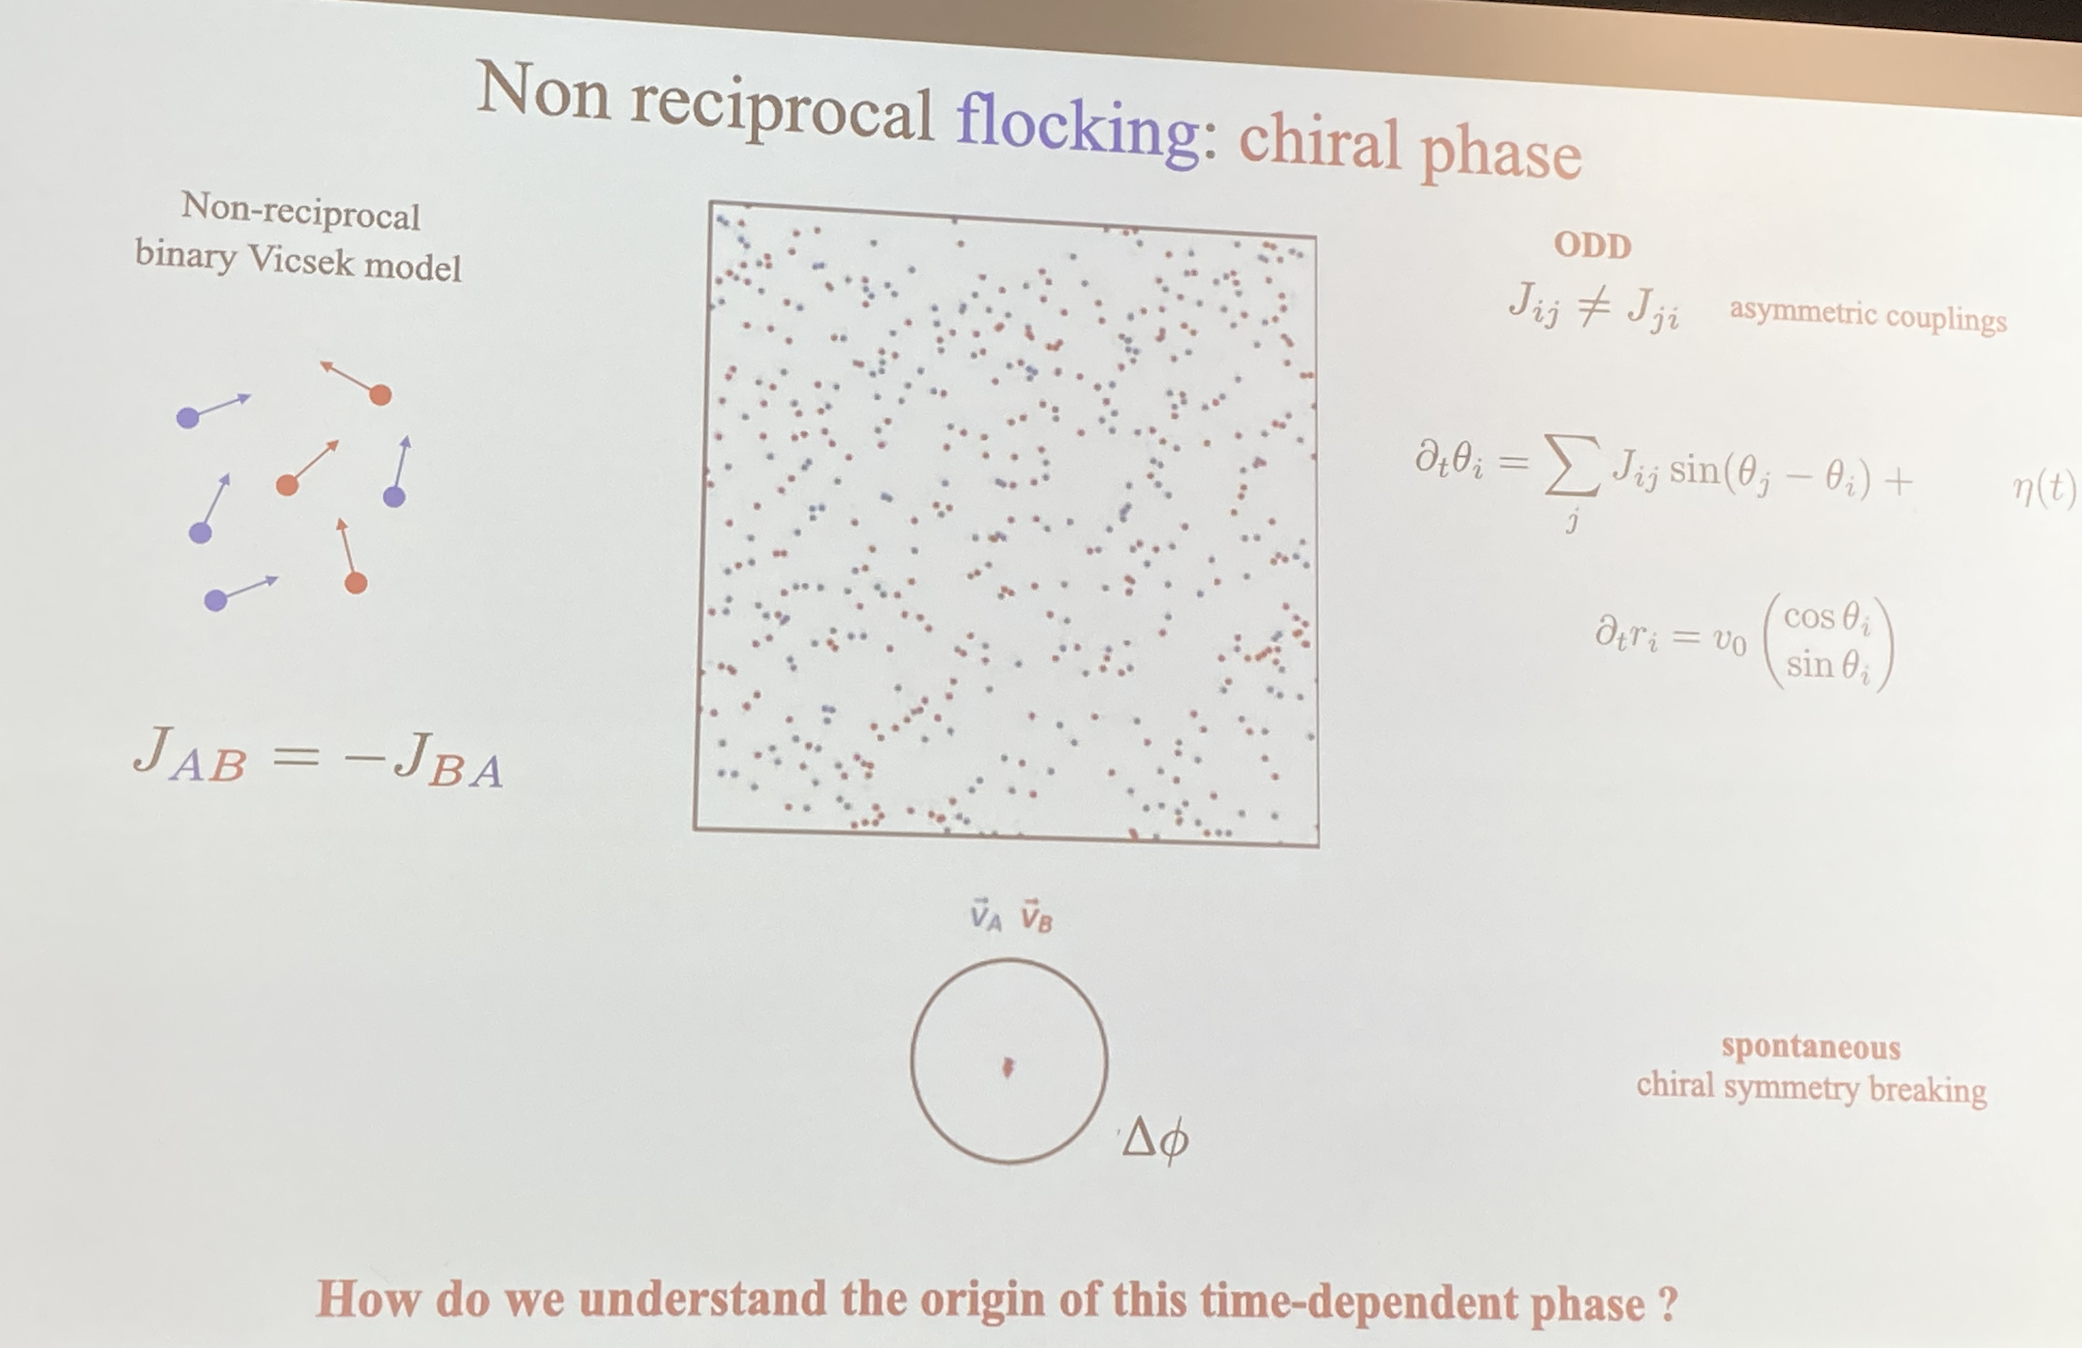
\includegraphics[scale=0.3]{Lectures/Images/lec18-flocking.png}
\end{center}
\begin{center}
    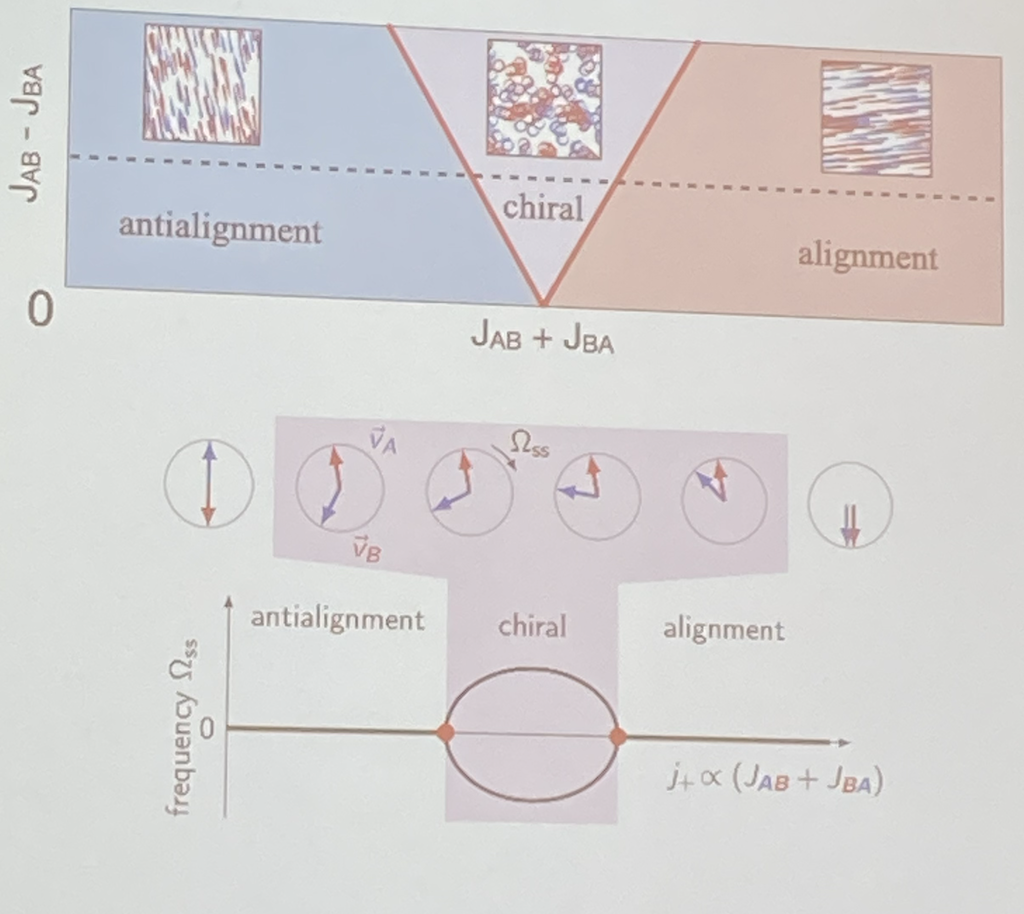
\includegraphics[scale=0.35]{Lectures/Images/lec18-flockingphases.png}
\end{center}

\subsection{Goldstone Modes, Comments on Non-Reciprocal Phase Transitions}

Note that in this problem we also have a Goldstone mode - a global rotation (the analog of translation on a line - here we have just put the entire system on a ring, so the translational Goldstone mode becomes a global rotational Goldstone mode). Usually, people talk about Goldstone modes as the rotation around the Mexican hat (here $\bar{\phi}$) and the oscillatory mode as the massive one (here $\Delta \phi$). At the exceptional point, the massive mode coalesces with the Goldstone one. 

\begin{center}
    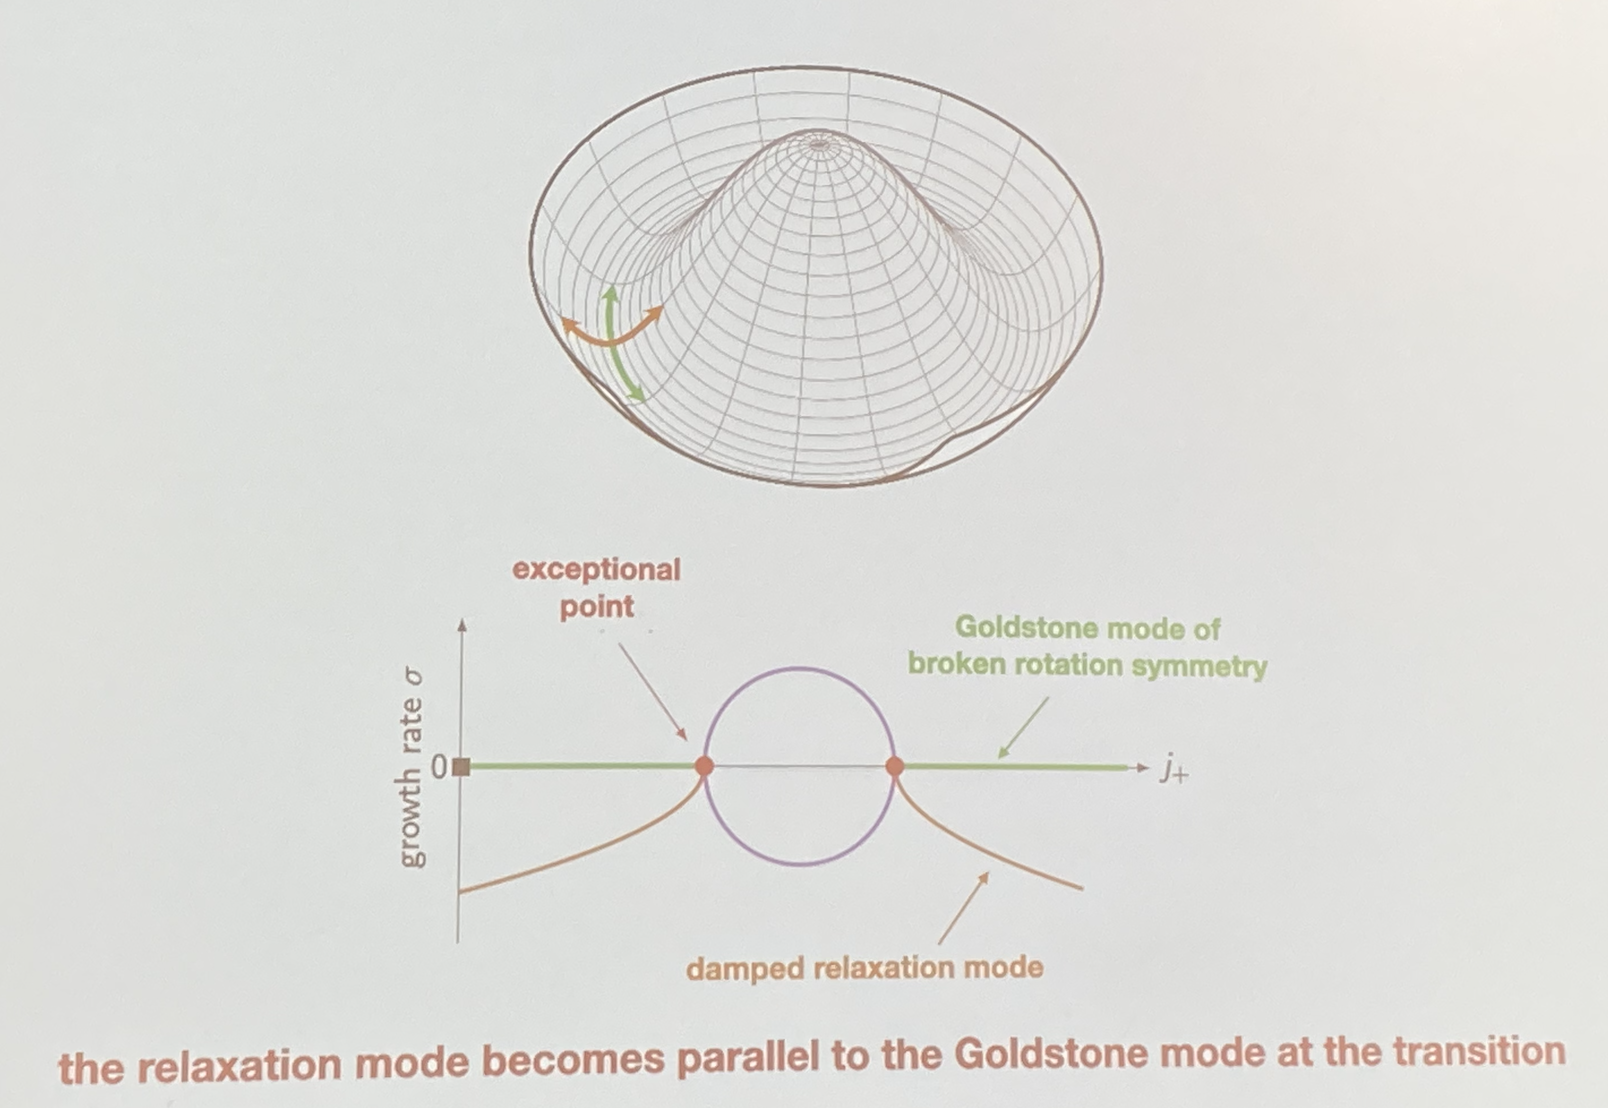
\includegraphics[scale=0.3]{Lectures/Images/lec18-goldstone.png}
\end{center}

Normally, people think about equilibrium phases as performing an optimization with $\p_t \phi = -\frac{\delta F}{\delta \phi}$. But, non-equilibrium forces also have a transverse component, and therein the cyclic dynamical states do not arise from any free energy minimization/variational mechanics. 

\begin{center}
    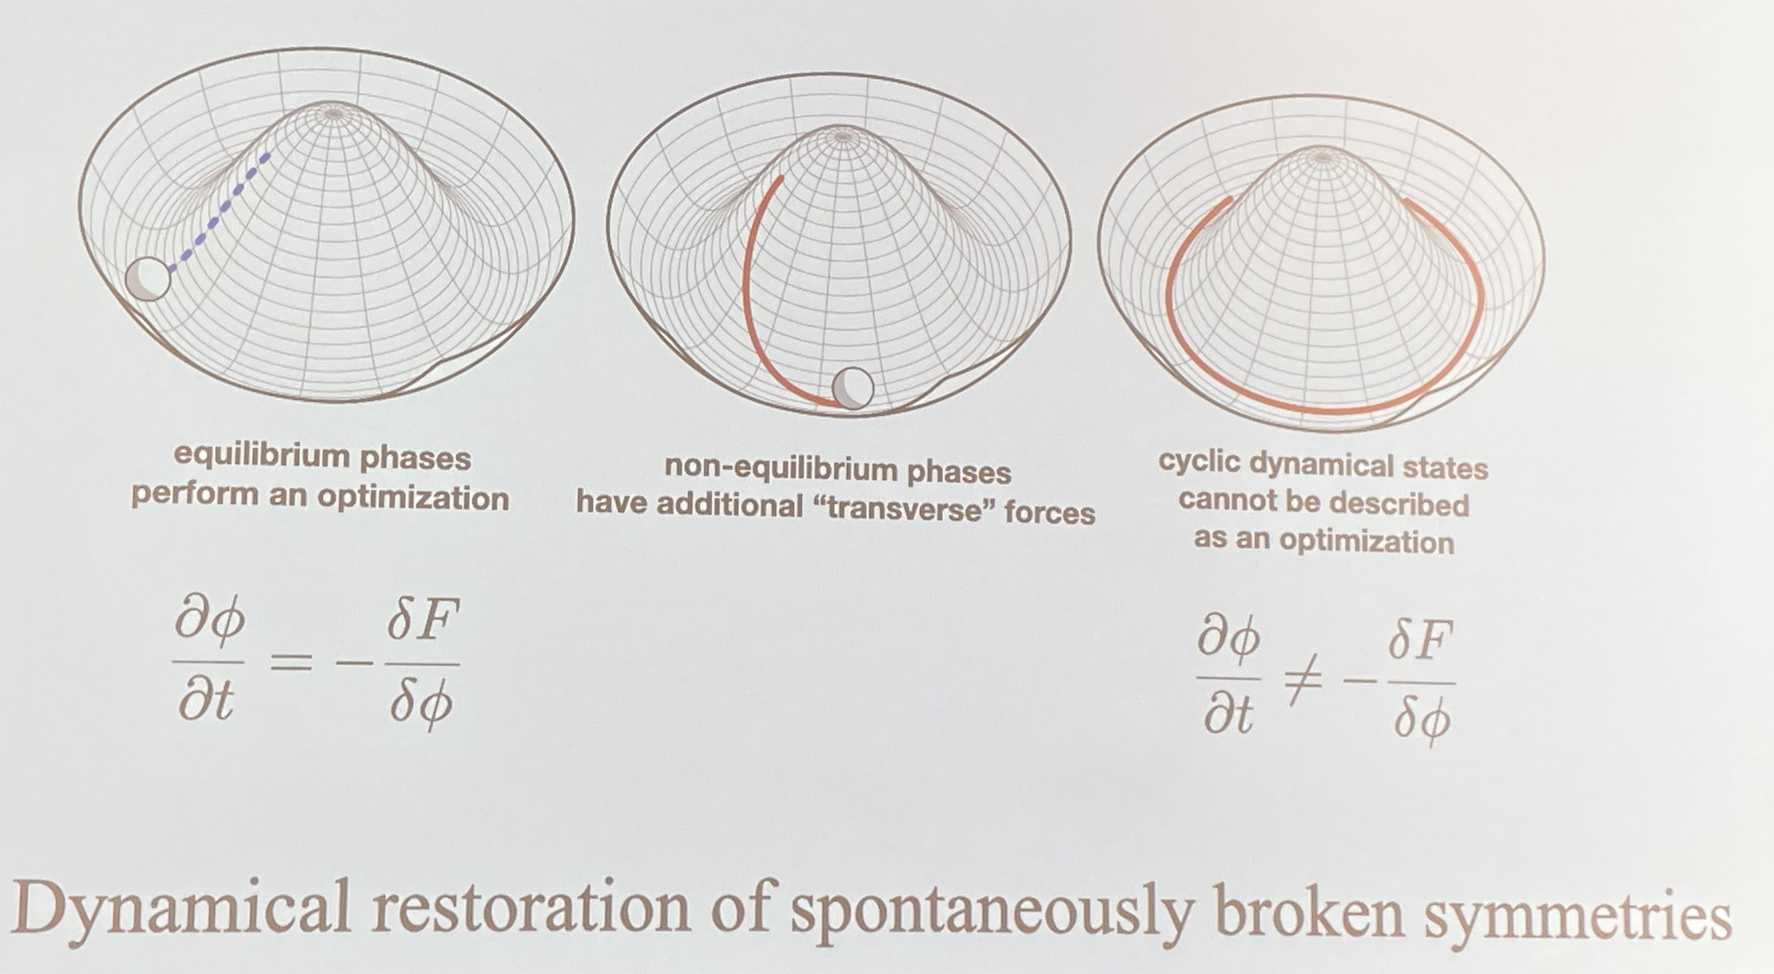
\includegraphics[scale=0.3]{Lectures/Images/lec18-nonvariational.png}
\end{center}

Such non-variational systems are quite ubiquotous, e.g. in biological systems, social dynamics or open quantum systems (where we lose unitarity) - indeed, most systems are, despite what the concentration of papers focusing on equilibrium systems may indicate.